\documentclass[problem]{mcs}

\begin{pcomments}
  \pcomment{FP_not_3_colors}
  \pcomment{excerpted from PS_coloring_no_triangles}
\end{pcomments}

\pkeywords{
  simple_graph
  coloring
}

%%%%%%%%%%%%%%%%%%%%%%%%%%%%%%%%%%%%%%%%%%%%%%%%%%%%%%%%%%%%%%%%%%%%%
% Problem starts here
%%%%%%%%%%%%%%%%%%%%%%%%%%%%%%%%%%%%%%%%%%%%%%%%%%%%%%%%%%%%%%%%%%%%%

\begin{problem}
Let $G$ be the graph of Figure~\ref{fig:Groetzsch}.  Prove
that $G$ is not 3-colorable.

\begin{figure}[hb]
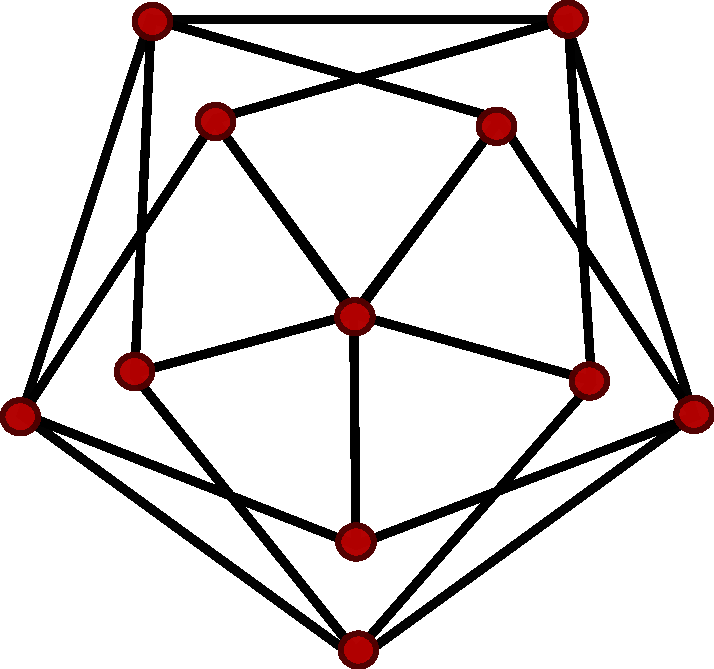
\includegraphics[width=1.6in]{coloring_no_triangles}
\caption{Graph $G$ with $\chi(G)>3$.}
\label{fig:Groetzsch}
\end{figure}

\begin{solution}
Assume by contradiction that there is one coloring using only 3
colors: red, blue and green.  The outer pentagon of the graph is an
odd-length cycle, and so requires all 3 colors.  So we can assume wlog
that the outer pentagon is colored as shown in the left hand side of
Figure~\ref{fig:coloring_no_triangles_solution2}.

This coloring of the pentagon forces the coloring of three interior
points, as shown in the right hand side of
Figure~\ref{fig:coloring_no_triangles_solution2}.  Now the point in
the center has neighbors with all three colors, so it is impossible to
color it.

\begin{figure}\inbook{[h]}
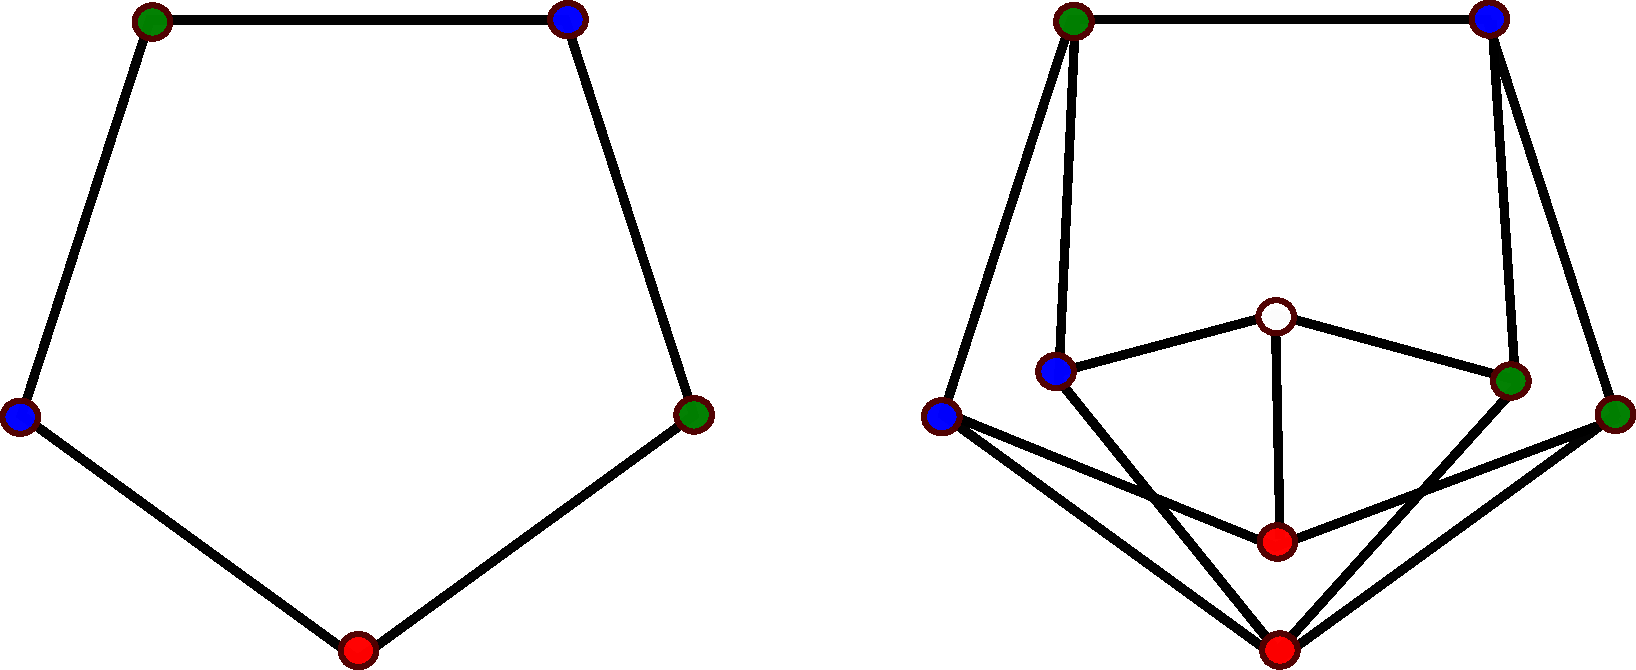
\includegraphics[width=4in]{coloring_no_triangles_solution2}
\caption{Constraints on a 3-coloring.}
\label{fig:coloring_no_triangles_solution2}
\end{figure}
\end{solution}

\end{problem}

%%%%%%%%%%%%%%%%%%%%%%%%%%%%%%%%%%%%%%%%%%%%%%%%%%%%%%%%%%%%%%%%%%%%%
% Problem ends here
%%%%%%%%%%%%%%%%%%%%%%%%%%%%%%%%%%%%%%%%%%%%%%%%%%%%%%%%%%%%%%%%%%%%%

\endinput
